\documentclass[10pt]{article}
\usepackage[paperwidth=190mm,paperheight=140mm,margin=7mm]{geometry}
\usepackage{fontspec,booktabs,multirow,amssymb,graphicx}
\usepackage[table]{xcolor}
\usepackage{tikz}
\setmainfont{TeX Gyre Termes}
\definecolor{sectiongray}{gray}{0.91}
\definecolor{selected}{RGB}{237,249,237}
\definecolor{quiet}{gray}{0.42}
\definecolor{gain}{RGB}{0,105,32}
\pagestyle{empty}\setlength{\parindent}{0pt}
\setlength{\tabcolsep}{4pt}\renewcommand{\arraystretch}{1.04}
\newcommand{\captext}[3]{\noindent Table #1: \textbf{#2} #3\par\vspace{5pt}}
\newcommand{\band}[2]{\rowcolor{sectiongray}\multicolumn{#1}{l}{\textit{#2}}\\}
\newcommand{\unc}[2]{#1\,{\scriptsize\textcolor{quiet}{$\pm$#2}}}
\newcommand{\yes}{$\checkmark$}
\newcommand{\no}{--}
\newcommand{\full}{
\begin{tikzpicture}[baseline=-.5ex]\path[use as bounding box] (-.89ex,-.89ex) rectangle (.89ex,.89ex);\filldraw[draw=black,fill=black,line width=.095ex] (0,0) circle[radius=.78ex];\end{tikzpicture}}
\newcommand{\emptyc}{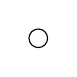
\begin{tikzpicture}[baseline=-.5ex]\path[use as bounding box] (-.89ex,-.89ex) rectangle (.89ex,.89ex);\draw[black,fill=none,line width=.095ex] (0,0) circle[radius=.78ex];\end{tikzpicture}}
\newcommand{\halfc}{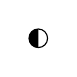
\begin{tikzpicture}[baseline=-.5ex]\path[use as bounding box] (-.89ex,-.89ex) rectangle (.89ex,.89ex);\fill[black] (0,.78ex) arc[start angle=90,end angle=270,radius=.78ex] -- cycle;\draw[black,line width=.095ex] (0,0) circle[radius=.78ex];\end{tikzpicture}}
\begin{document}
\captext{4}{Sensitivity to model and inference settings.}{One factor varies in each panel; all other settings remain at the gray default. Accuracy (\%) and latency (ms) are synthetic. Bold marks the best value within each panel and column.}
\vspace{3pt}
\begin{minipage}[t]{.24\linewidth}\centering\setlength{\tabcolsep}{3pt}
\begin{tabular}{@{}rrr@{}}\toprule
Blocks & Acc.$\uparrow$ & ms$\downarrow$ \\
\midrule
6 & 78.2 & \textbf{8.1} \\
\rowcolor{sectiongray}
12 & 80.4 & 10.2 \\
18 & 81.1 & 13.8 \\
24 & \textbf{81.3} & 17.6 \\
\bottomrule\end{tabular}\par\smallskip\raggedright (a) \textbf{Model depth.}\end{minipage}
\hfill
\begin{minipage}[t]{.24\linewidth}\centering\setlength{\tabcolsep}{3pt}
\begin{tabular}{@{}rrr@{}}\toprule
Slots & Acc.$\uparrow$ & ms$\downarrow$ \\
\midrule
16 & 78.9 & \textbf{9.3} \\
\rowcolor{sectiongray}
32 & 80.4 & 10.2 \\
64 & 81.0 & 12.6 \\
128 & \textbf{81.2} & 16.1 \\
\bottomrule\end{tabular}\par\smallskip\raggedright (b) \textbf{Memory size.}\end{minipage}
\hfill
\begin{minipage}[t]{.24\linewidth}\centering\setlength{\tabcolsep}{3pt}
\begin{tabular}{@{}rrr@{}}\toprule
Frames & Acc.$\uparrow$ & ms$\downarrow$ \\
\midrule
8 & 77.1 & \textbf{6.8} \\
16 & 79.2 & 8.4 \\
\rowcolor{sectiongray}
32 & 80.4 & 10.2 \\
64 & \textbf{80.9} & 14.8 \\
\bottomrule\end{tabular}\par\smallskip\raggedright (c) \textbf{Context length.}\end{minipage}
\hfill
\begin{minipage}[t]{.24\linewidth}\centering\setlength{\tabcolsep}{3pt}
\begin{tabular}{@{}rrr@{}}\toprule
Top-k & Acc.$\uparrow$ & ms$\downarrow$ \\
\midrule
1 & 78.6 & \textbf{8.7} \\
2 & 79.7 & 9.2 \\
\rowcolor{sectiongray}
4 & 80.4 & 10.2 \\
8 & \textbf{80.8} & 12.4 \\
\bottomrule\end{tabular}\par\smallskip\raggedright (d) \textbf{Retrieval budget.}\end{minipage}

\end{document}
